\section{System Architecture}
\label{sec:system}

\begin{figure}[t]
    \centering
    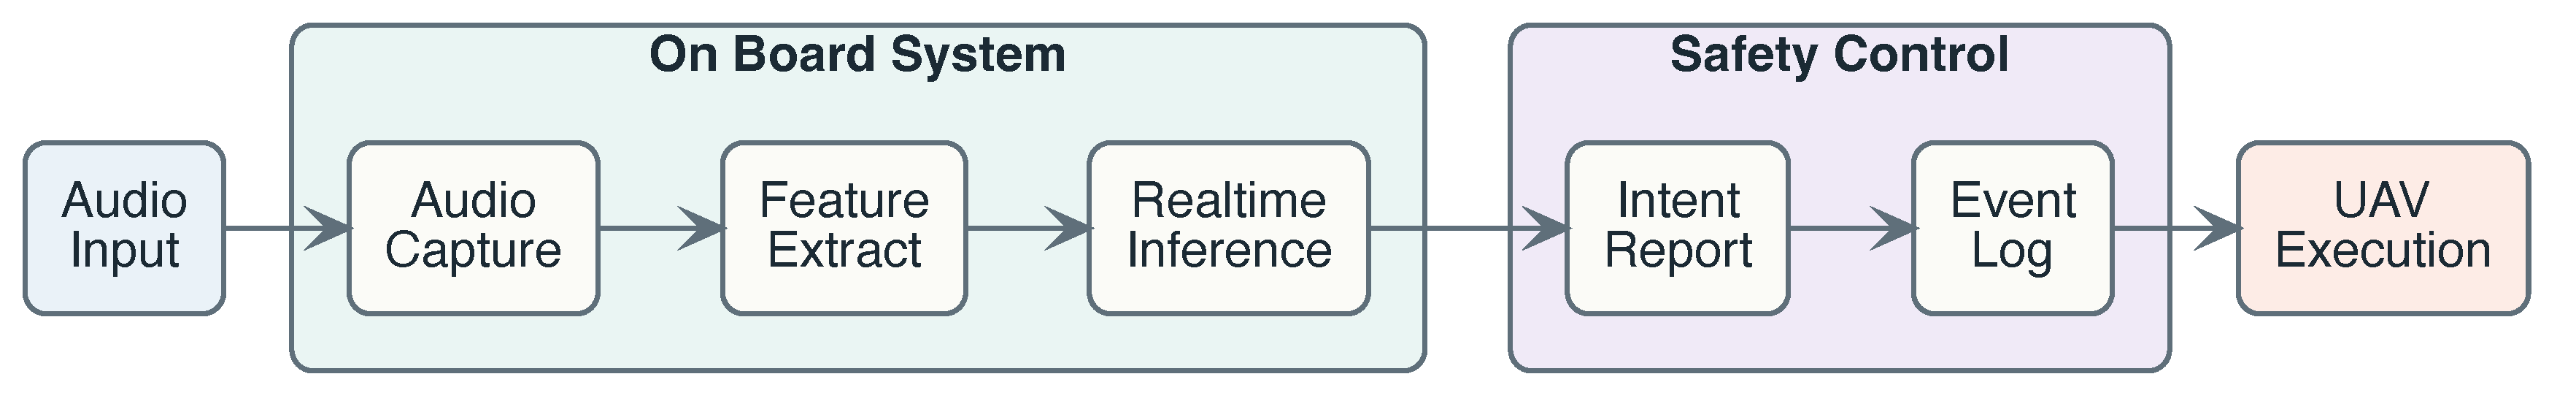
\includegraphics[width=\columnwidth]{figures/system_architecture.pdf}
    \caption{\sys{} system architecture. Rotor-noisy nearby speech is mapped into a safety-relevant intent state and admitted to vehicle-facing decision logic only through the safety-state boundary, separating recognition from vehicle-facing action.}
    \label{fig:system_architecture}
\end{figure}

\begin{table}[t]
    \centering
    \caption{Intent-state mapping used by \sys{}. Each short audio window is mapped to a safety-relevant intent state; low-confidence predictions are handled as unknown.}
    \label{tab:intent_state_mapping}
    \footnotesize
    \setlength{\tabcolsep}{3pt}
    \begin{tabular}{@{}p{0.22\linewidth}p{0.33\linewidth}p{0.35\linewidth}@{}}
        \toprule
        Intent state & Speech meaning & Boundary handling \\
        \midrule
        Emergency
        & Safety-related speech.
        & Prioritize safe response by boundary rules. \\
        Movement
        & Ordinary control speech.
        & Keep pending for authority and state checks. \\
        Unknown
        & Uncertain audio.
        & Log and map to no action. \\
        \bottomrule
    \end{tabular}
\end{table}


\subsection{Voice as a Safety Interaction Layer}

\sys{} sits between nearby human speech and the UAV control stack. It is not a replacement for obstacle avoidance, geofencing, failsafe landing, manual override, or the flight controller. Those mechanisms continue to monitor the vehicle, the environment, and the operator channel. \sys{} adds a different input: a local voice channel for people near the drone, especially when using a phone or controller is slow, awkward, or unavailable.

The architectural design is to keep this voice channel narrow. Each speech window is first converted into a safety-relevant intent state, not a flight command. The report records what the voice layer believes it heard, how confident it was, and when the intent state was produced. Only after that record exists does a safety-state boundary decide whether the state should be ignored, held, escalated, or forwarded to a downstream execution path. Figure~\ref{fig:system_architecture} shows this separation, and Table~\ref{tab:intent_state_mapping} expands the intent-state mapping.

The separation between the recognizer and the UAV-facing interface is central to maintaining the safety boundary. A conventional command recognizer can be evaluated by whether it selects the right spoken term. A UAV voice interface also has to ask what happens after the term is recognized. By turning speech into an intent state first, the system gives the control side a point where it can check vehicle state, operator authority, recent history, and existing safety mechanisms before any action is considered.

The pipeline has six stages. The microphone on the drone captures a short audio window. The acoustic frontend converts that window into log-mel features. The recognizer estimates whether the window expresses emergency speech, ordinary movement-oriented speech, or unsupported/uncertain audio. The intent-state reporter attaches confidence and timing fields. The safety-state boundary checks the reported state against the current interaction state, authority, and configured boundary rules. Only after that boundary can a gated vehicle-facing action be considered. Each stage is observable, which lets the evaluation separate recognition quality, embedded runtime, reporting behavior, boundary behavior, and vehicle-facing command behavior.

The intent-state representation is the point where the speech system becomes a UAV systems component. A conventional speech interface often passes a word, phrase, or command string to the application. \sys{} instead passes a typed intent-state record. The record contains the intent state, confidence, sequence or timing information, and the status needed to interpret whether the embedded path was operating normally. This makes the voice layer inspectable: if the system behaves incorrectly, the log can show whether the error came from acoustic recognition, state reporting, boundary-rule handling, or a downstream vehicle-facing interface.

The safety-state boundary is also where \sys{} remains compatible with existing safety mechanisms. Obstacle avoidance, geofencing, battery state, link status, manual override, and mission constraints can all be checked after a voice intent state is produced. The boundary then decides whether any gated vehicle-facing response may be forwarded. The voice layer does not need to know the full vehicle-state and authority model. It needs to provide a small, reliable observation that the boundary can combine with the rest of the vehicle state. This division keeps the speech model from becoming the authority for physical action.

\subsection{Intent States and Safety-State Boundary}

The voice layer exposes a small intent-state mapping to the rest of the system. It does not expose a long command grammar or natural-language plan. The mapping contains three visible intent states: emergency, movement, and unknown. This choice is deliberately conservative. It gives the system enough information to distinguish safety-critical speech from ordinary interaction, while also reporting confidence so that boundary rules can contain unsupported or uncertain audio.

Table~\ref{tab:intent_state_mapping} describes system semantics: it says what the voice layer is allowed to communicate about the speaker's intent, not what the drone must immediately do.

Emergency is the safety-critical intent state. It is useful because it can make the voice channel responsive to nearby human concern, but it is still an inferred state rather than proof of a hazard. The safety-state boundary can decide whether to hold position, stop a task, escalate to an operator, or request confirmation, depending on the UAV state and the surrounding safety inputs.

Movement represents ordinary voice interaction. It indicates that the speech may be control-oriented, but it does not contain a direction, distance, velocity, or permission. The boundary must still decide whether any movement-related response is allowed by authority, vehicle-state, and safety checks. This prevents the recognizer from becoming a direct speech-to-navigation interface.

Unknown is the containment mechanism. It covers unsupported phrases, background sounds, and ambiguous speech. The same path can also be used by boundary rules for low-confidence recognizer outputs. In a physical system, this no-action path matters as much as a positive class: the voice channel must be able to say that the audio should not influence the drone.

The boundary applies the same logic over time. Each intent-state update is associated with a short validity window so that stale speech does not remain actionable. Repeated updates can be suppressed, rate-limited, or used as confirmation according to configured boundary rules. The boundary can also require additional context before forwarding a response: for example, a movement update may require manual authority, a safe vehicle state, and an allowed operating region, while an emergency update may bypass ordinary interaction handling but still enter a controlled hold or escalation path. These temporal, authority, vehicle-state, and safety checks are part of the safety interaction layer, not after-the-fact implementation details.

This design also makes failures easier to interpret. A missed emergency is an acoustic failure. A movement update forwarded without authorization is a boundary failure. An unknown update that becomes a command is a mapping failure. Separating these cases is important for evaluation because a single end-to-end success rate would hide which layer needs to be improved.

\subsection{End-to-End Walkthrough}

Consider a person standing near a small UAV during a low-altitude task. The person speaks a short utterance such as ``stop,'' a movement-like request, or an unrelated phrase. The microphone captures a one-second window that includes both speech and rotor self-noise. The recognizer does not try to recover a transcript. It produces one of the three intent states with a confidence score.

If the update is emergency, the safety-state boundary records it, checks the current UAV state, and routes it to the safety-critical handling path according to the active confidence setting and configured boundary rules. The resulting behavior may be a hold, stop, escalation, or confirmation request, depending on those rules. If the update is movement, the boundary records it as an ordinary interaction request and keeps it pending until authority, vehicle-state, and safety checks allow a movement-related response. If the update is unknown, or if a future threshold rule treats the update as too uncertain, the boundary logs it and takes no control action. Only after these checks can an implementation forward a gated vehicle-facing action.

This walkthrough illustrates why the architecture is not just a recognizer attached to a drone. The recognizer supplies a constrained observation. The safety-state boundary decides what that observation means for the current state of the vehicle. The log connects the two, so later analysis can tell whether a failure came from acoustic recognition, intent-state delivery, boundary-rule handling, or a downstream vehicle-facing path.

The same walkthrough also explains the role of latency. A slow recognizer reduces the usefulness of voice interaction, but a fast recognizer is not sufficient unless the intent-state update reaches the safety-state boundary with the right state information. The response-time decomposition therefore separates capture, feature extraction, board-side model invocation, intent-state reporting, boundary decision, gated action forwarding, and acknowledgement. This decomposition keeps the system claim precise: \sys{} is an intent-state mediation pipeline whose timing and control handling are visible at each stage.
